\documentclass{article}[12pt,a4paper]

%!TEX root = main.tex

\def\finex{{\unskip\nobreak\hfil
\penalty50\hskip1em\null\nobreak\hfil{\Large $\diamond$}
\parfillskip=0pt\finalhyphendemerits=0\endgraf}}

\newenvironment{lmref}[1]{%
	\vspace*{0.3cm}
	\noindent {\bf  Lemma #1.}}

\newenvironment{thref}[1]{%
	\vspace*{0.3cm}
	\noindent {\bf  Theorem #1.}}

\newenvironment{corref}[1]{%
	\vspace*{0.3cm}
	\noindent {\bf  Corollary #1.}}


\newcommand{\picalc}{$\pi$-calculus~}
\newcommand{\ms}[1]{\mathsf{#1}}
\newcommand{\ctx}{\mathtt{C}}
\newcommand{\co}[1]{\overline{#1}}
\newcommand{\proj}[1]{\mathtt{proj}(#1)}
\newcommand{\projs}[1]{\mathtt{proj_n}(#1)}
\newcommand{\lts}[1]{\xrightarrow{#1}}
\newcommand{\comm}[1]{\textcolor{blue}{#1}}
\newcommand{\red}[1]{\textcolor{red}{#1}}
\newcommand{\key}{\mathtt{keys}}
\newcommand{\flts}[1]{\overset{#1}\twoheadrightarrow}
\newcommand{\rev}{^{\bullet}}
%\newcommand{\forw}{_{\twoheadrightarrow}}
\newcommand{\eq}{\sim} 
\newcommand{\env}{\theta} 
\newcommand{\ex}{e} 
\newcommand{\proc}[3]{\langle #1,#2,#3\rangle } 
\newcommand{\erl}[1]{\hookrightarrow_{#1}} 
\newcommand{\mem}[2]{[#1\;;#2]}
\newcommand{\bl}[1]{\textcolor{blue}{#1}}
\newcommand{\rd}[1]{\textcolor{red}{#1}}
\newcommand{\mtt}[1]{\mathtt{#1}}
\newcommand{\pid}{\mathtt{pid}}
\newcommand{\procl}[4]{\langle #1,#2,#3,#4\rangle } 
\newcommand{\con}{\equiv}
\newcommand{\conk}{\equiv_k}
\newcommand{\extcon}{\equiv_c}
\newcommand{\de}{\delta}
\newcommand{\G}{\Gamma}
\newcommand{\logg}[1]{\rightharpoonup_{#1}}
\newcommand{\rlogg}[1]{\leftharpoondown_{#1}}
\newcommand{\la}{\lambda}
\newcommand{\col}[1]{\mathtt{col}(#1)}
\newcommand{\rel}{\mathcal{R}}
\newcommand{\conc}{\smile_c}
\newcommand{\nil}{{\bf{0}}}
%\newcommand{\res}{\nu}
\newcommand{\res}[1]{\nu #1\,}
\newcommand{\out}[1]{\langle #1\rangle}
\newcommand{\cont}{\triangleright}
\newcommand{\sub}[2]{\{#1/#2\}}
\newcommand{\op}{op_n}
\newcommand{\pidd}{Pid}
\newcommand{\fmod}{\rightarrowtail}
\newcommand{\enc}[1]{\llparenthesis #1 \rrparenthesis}
\newcommand{\blt}{\bullet}
\newcommand{\str}{C}
\newcommand{\term}[1]{T[#1]}
\newcommand{\en}[1]{\Lbag #1 \Rbag}
\newcommand{\signal}[1]{\{ #1\}}
\newcommand{\systset}{\mathbb{S}}
\newcommand{\confset}{\mathbb{C}}
\newcommand{\set}[1]{\{ #1\}}
\newcommand{\node}[3]{#1,#2\mkern-3mu:\mkern-3mu[\mkern-6mu[#3]\mkern-6.2mu]}


\usepackage{listings}
\usepackage[version=3]{mhchem} % Package for chemical equation typesetting
\usepackage{siunitx} % Provides the \SI{}{} and \si{} command for typesetting SI
% units
\usepackage{fancyvrb}
\usepackage[hidelinks]{hyperref}
\usepackage{breakurl}             % Not needed if you use pdflatex only.
\usepackage{underscore}           % Only needed if you use pdflatex.
\usepackage{microtype}%if unwanted, comment out or use option "draft"
\usepackage{amssymb}
\setcounter{tocdepth}{3}
\usepackage{graphicx}
\usepackage{listings}
\usepackage{color}
\usepackage{rotating}
\usepackage{todonotes}
\usepackage{mathpartir}
\usepackage{url}
\usepackage{tikz}
\usepackage{amsmath}
\usepackage{stmaryrd}
\usepackage{amsthm}
\usepackage{float}
\usepackage{hyperref}
\usepackage{thm-restate}
\usepackage{caption}
\captionsetup[figure]{font=small,labelfont=small}
\usetikzlibrary{matrix}


\renewcommand{\labelenumi}{\alph{enumi}.} % Make numbering in the enumerate environment by letter rather than number (e.g. section 6)

\theoremstyle{definition}
\newtheorem{example}{Example}[section]
\newtheorem{theorem}{Theorem}
\newtheorem{lemma}{Lemma}
\newcommand{\paral}{\;|\;}
\newcommand{\cons}{\mbox{:}}

\usetikzlibrary{calc,decorations.pathmorphing,shapes}
\newcounter{sarrow}
\newcommand\blts[1]{%
  \stepcounter{sarrow}%
  \mathrel{\begin{tikzpicture}[baseline= {( $ (current bounding box.south) + (0,-0.5ex) $ )}]
      \node[inner sep=.5ex] (\thesarrow) {$\scriptstyle #1$};
      \path[draw,<-,decorate,
      decoration={zigzag,amplitude=1.2pt,segment length=1.5mm,pre=lineto,pre length=6pt}]
      (\thesarrow.south east) -- (\thesarrow.south west);
    \end{tikzpicture}}%
}

\newcommand{\footremember}[2]{%
    \footnote{#2}
    \newcounter{#1}
    \setcounter{#1}{\value{footnote}}%
}
\newcommand{\footrecall}[1]{%
    \footnotemark[\value{#1}]%
} 

\begin{document}

\title{Generation of a Reversible Semantics for Erlang in Maude (Technical Report)}

\author{Giovanni Fabbretti\footremember{Gre}{Univ. Grenoble Alpes, INRIA, CNRS,
    Grenoble INP, LIG, France}, Ivan Lanese\footremember{Bol}{Focus Team, Univ. of Bologna/INRIA, Italy}, Jean-Bernard Stefani\footrecall{Gre}}
\date{}

\maketitle % typeset the header of the contribution 

\abstract{
  In recent years, reversibility in concurrent settings has
  attracted quite some interest thanks to its many applications in
  different areas, like error-recovery, debugging, biological
  systems. It has been investigated in formalisms such as
  Petri nets, process algebras and real programming languages.
  Nonetheless, all the attempts made so far suffer from the same
  limitation: they have been devised ad-hoc. To address this limit
  Lanese et al.~have recently proposed a novel general method to derive
  a concurrent reversible semantics starting from a non-reversible one. The
  general method though lacks an implementation that proves its
  feasibility in practice. The aim of this work is to provide such an
  implementation and to apply it to a case study on the Erlang
  programming language. }

\section{Introduction}


Reversibility is the capability to execute a program both in a forward
and backward manner. While reversibility is well-understood for
sequential systems the same cannot be said for concurrent
ones. Indeed, in sequential systems, actions can be undone in reverse
order of completion.  The major difficulty when reversing the
execution of a concurrent system is that the order of actions is no
more a total order, since execution of concurrent actions may overlap.
To tackle this problem Danos and Krivine in~\cite{DanosK04} propose a
notion of \emph{causal-consistent reversibility}, which aims at
establishing a way to undo actions in concurrent systems. Causal
consistency states that an action can be undone iff all its
consequences, if any, have been undone beforehand. Notably, this
definition does not need a (temporal) total order of actions, but
builds on a notion of causality.

Following their seminal work, reversibility has been studied in other formalisms
as well, such as: CCS~\cite{DanosK04,PhillipsU07}, $\pi$-calculus~\cite{CristescuKV13}, higher-order $\pi$-calculus~\cite{LaneseMS16},
$\mu$Klaim~\cite{GiachinoLMT17}, Petri nets~\cite{PhilippouP18,MelgrattiMU20}, etc.

Another stream of research, investigating reversibility as a debugging technique for concurrent systems,
has risen after \cite{GiachinoLM14}, where Giachino et al.~proposed to
equip a concurrent debugger with reversible primitives.
The approach proposed by Giachino et al.~has subsequently been applied in the context of a real programming language, namely Erlang~\cite{LaneseNPV18,Lanese0PV18,Gonzalez-AbrilV21,FabbrettiLS21}.

However, as anticipated, all the works cited so far suffer from the same limitation: reversibility has always been
devised manually. Given a forward non-reversible semantics, the authors manually
derived an extension of its forward semantics, enabling reversibility, and the corresponding backward semantics, defining reverse execution.
Deriving a reversible semantics manually presents some limitations: the
process is error-prone, it does not scale well to other formalisms, and lacks
uniformity - i.e., the same properties must be proved for each formalism.

To address this problem, Lanese and Medic~proposed in~\cite{LaneseM20} a
general method to
automatically derive a causal-consistent reversible semantics starting from a non-reversible one. The
advantages of having an automatic method are symmetric to the disadvantages
listed above, i.e., the method: is not error-prone; scales well; is uniform. The key idea behind the general method is to capture
causal dependencies, needed for the definition of causal-consistent reversibility, in terms of resources consumed and produced. The non-reversible
semantics taken in input must be a reduction semantics and the entities on the
left-hand side of a rule are seen as the resources to be \emph{consumed} to
\emph{produce} the resources on the right-hand side - i.e., the new entities.
As an example, even without knowing the details that will be explained later on, let
us consider the following reduction. 
\begin{equation}\label{samplerule}
\langle p_1, \theta, p_2~\ms{!}~hello, me\rangle \rightarrow \langle p_1, \theta,
hello, me\rangle \paral\langle p_1, p_2,hello \rangle
\end{equation}
On the left we have a process $p_1$ ready to send a
message ($p_2~\ms{!}~hello$ requires to send atom $hello$ to process $p_2$). When the reduction is executed the process is consumed to produce the message
$\langle p_1, p_2,hello \rangle$ and the evolution of the process itself after the send.

In order to define the reversible semantics, we need two ingredients: keys and memories.
Keys are attached to entities, so to distinguish entities with the same form but different history.
Memories are used to track past states, that would normally be lost during the computation, so that
they can be restored during backward execution.

In~\cite{LaneseM20} the approach is only described theoretically and
no implementation is provided. Actually, the method relies on
reversing instances of rules such as the one above, which are infinitely many in almost any
non trivial formalism, which makes not immediately clear that an
implementation could exist. Our work aims at showing that indeed the
method can be implemented and used in practice.  The key idea here is
that the instances of rules can be captured by a finite (and
frequently small) number of rule schemas, and the approach can be
applied to schemas. In order to do this, we use Maude~\cite{maude} to represent the reduction semantics (both the non-reversible one in input and the reversible one we generate) as well as for the tool generating the reversible semantics.
To further prove the practicality of the
approach, we apply it to a case study on the Erlang programming
language.

The main contributions of this work are:
\begin{itemize}
  \item a novel formalization of Erlang semantics using
    Maude;
  \item the implementation of a tool that automatically derives a reversible
    semantics starting from a non reversible one.
\end{itemize}

The rest of this report is structured as follows. We provide the reader with the required
background in Section~\ref{sec:background}. In
Section~\ref{sec:formalizing-erlang} we present the formalization of
the Erlang semantics in Maude and in Section~\ref{sec:generating} we discuss how the reversible semantics
is generated. In Section~\ref{sec:ongoing-work} we give some hints on the correctness of the reversible semantics. Finally, in Section~\ref{sec:conclusion} we give some
conclusion and we hint at possible future directions.

All the code discussed in this report is publicly available
at~\cite{erl-maude-repo}. 

\section{Background}\label{sec:background}

\subsection{Erlang: Syntax and Semantics}

Erlang is a functional and concurrent programming language. First
introduced in 1986 by Ericsson, it has gained quite a lot of
popularity since then.  Today it is widely used and mostly appreciated
because it is easy to learn, provides useful abstractions for
concurrent and distributed programming, and because of its support for
highly-available systems. Erlang implements the actor model~\cite{Hewitt73}, a
concurrency model based on message passing. In the actor model, each
process is an actor that can interact with other actors
only through the exchange of messages, no memory is shared. Indeed,
central in Erlang are the $\ms{send}$, $\ms{receive}$ and $\ms{spawn}$
operations, to, respectively, send a message, receive a message, and
create a new actor. Actors are identified by a unique pid (process identifier) and have a queue of messages which have arrived but have not yet been processed.
An actor evaluates an expression, and has an environment to store variable bindings.

The rest of this section provides the reader with a basic understanding
of the Erlang programming language. We begin by illustrating its syntax, depicted in
Fig.~\ref{ErlangSyntax}\footnote{We support the functional and concurrent fragment of the
  Erlang language.}. 

An Erlang program can be seen as a collection of modules, where a module is a sequence of function definitions. Each function is uniquely identified by its name and by the
number of formal parameters. Each function may be specified by cases via multiple definitions. The correct definition for each invocation is selected by pattern matching on parameters. The body of each definition is represented
by a sequence of expressions. In the following we denote an expression with $e$
and sequences of expressions as $e_1,\ldots,e_n$  - sequences of other
syntactical elements are represented in the same manner.  

Ground values in Erlang are: atoms (which are identifiers that either
begin with a lowercase or are enclosed by quotes), integers and
strings, as well as compositions of values using tuple and list
constructs. We range over ground values using $v$. Tuples are denoted
as $\{v_1,\ldots,v_n\}$ and lists are denoted as
$[v_1|v_2]$, where $v_1$ is the head and $v_2$ the tail.


\begin{figure}[t]
  \begin{center}
    $
    \begin{array}{rcl@{~~~~~~}l}

      program & ::= & mod_1  \dots  mod_n \\
      mod & ::= & fun\_def_1  \dots fun\_def_n  \\
      fun\_def & ::= & Atom([patterns]) \to exprs.\\
      pat & ::= & b\_value \mid Var \mid ~'\{'[patterns]'\}' \mid ~
                  '['[patterns|patterns] ']'\\
      patterns & ::= & pat ~\{ ','patterns\} \\
      exprs & ::= & expr ~\{ ',' exprs\} \\
      expr & ::= & b\_value \mid Var \mid ~'\{'[exprs]'\}' \mid ~'[' [exprs|expr] ']' \\
                    & \mid & \ms{case}~expr~\ms{of}~clseq~\mathsf{end} \mid
                             \ms{receive}~clseq~\mathsf{end} \mid expr ~ ! ~ expr \\
                    & \mid & pat = expr \mid
                             [Mod\cons]expr([exprs]) \\
      b\_value & ::= & Atom \mid Char \mid Float \mid Integer \mid String \\
      clseq & ::= & pat  \to exprs ~ \{ ';' pat \to exprs  \} \\
    \end{array}
    $
  \end{center}
  \caption{Language syntax} \label{ErlangSyntax}
\end{figure}

Variables can store ground values. Variables, e.g., $X,Age$, start with a capital letter and
are not enclosed in quotes.
Patterns, denoted by $pat$, are like the ground values,
but also admit the presence of variables. Patterns are used for pattern matching in the following contexts: (i) in the matching operation $e_1 = e_2$, (ii) in case statements $\ms{case}~e~\ms{of}~pat_1 \rightarrow exprs_1; \ldots; pat_n
\rightarrow exprs_n~\ms{end}$ to choose the branch
to evaluate according to the shape of the incoming data,
(iii) in receive
statements $\ms{receive}~pat_1 \rightarrow exprs_1; \ldots; pat_n
\rightarrow exprs_n~\ms{end}$, to analyze the shape of the received message, and
(iv) in function
definitions, to give values to the formal parameters. 

We start by explaining the match operation, $e_1 = e_2$. First, the expression $e_2$ on
the right-hand side is evaluated until it becomes a ground value,
occurrences of free variables, if any, raise an exception (however we do not support exception propagation and management in this work).
Then, the expression on the left-hand side, $e_1$, is evaluated until
it becomes a pattern, or a ground value in case no free variables
occur in it. Then the
two elements are matched against each other. Each free variable of the
left-hand side is bound to the corresponding ground value of the right-hand
side, ground values in corresponding position should coincide: if a mismatch occurs then an exception
is raised. If no mismatch occurs then the operation evaluates to the ground
value of the right-hand side and the environment is updated with the new bindings.

In the $\ms{case}$ construct, the expression $e$ must evaluate to a ground value, then it is matched against the patterns, from
top to bottom, until one that matches is found. When a match is found the environment
is enriched with the new bindings and the corresponding sequence of expressions evaluated, if
no match is found an exception is raised.

The behavior of the $\ms{receive}$ is similar to the one of the
$\ms{case}$, with the only difference that messages in the queue of
the process are tried as ground values till the match succeeds.
When a match is found the corresponding branch
is selected.  Contrary to the $\ms{case}$, if no match is found
then the process suspends.

Despite being - mostly - functional Erlang
admits some imperative operations that produce side-effects, like the $\ms{receive}$
above, spawning a new process, and sending a message. 

The syntax of message send is $e_1!e_2$, where $e_1$ must
evaluate to the pid of the receiver process and $e_2$ must evaluate to the ground value that represents the payload of the message. The expression itself evaluates to
the payload and, as a side-effect, the message is sent.

The $\ms{spawn}$ primitive creates a new process; it takes as argument
the function $f$ that the new process will execute, together with the
parameters for $f$ - if any. The spawn returns the
(fresh) pid of the newly created process and, as a side effect, the new process is created.

Finally, the function $\ms{self}$ returns the pid of the process
who invoked it.

%Self, send, spawn and receive are the concurrent features, offered by Erlang, that we support in this work.

\subsection{Maude}\label{sec:maude}

Maude~\cite{maude} is a programming language that efficiently implements rewriting logic~\cite{MeseguerMS96}.
Formally, a rewriting logic is a tuple $(\Sigma, E, R)$, where $\Sigma$
represents a collection of typed operators, $E$ a set of equations among the operators, and $R$ a set of
semantics rules.

Using a rewriting logic is quite convenient to formalize the
semantics of a language as it provides the benefits of using both an equational theory and rewriting rules.

On the one hand, the equational side of rewriting logic is well-suited to define the deterministic part of the model, where
we define equivalence classes over terms. More precisely we say that two terms
$v$ and $u$ are equivalent if under a set of equations $E$ we can prove $E \vdash
v = u$. Equations can be conditional and conditions can be either the
membership of the term to some kind or other equations.

% Rules
On the other hand, the rewriting rules are well-suited to define the
concurrent (non-deterministic) part of the programming language
semantics. The set of rules $R$ specifies how to rewrite a
(parameterized) term $t$ to another term $t'$.  Rewriting rules, like
equations, can be conditional and conditions can be
memberships, equations, as well as other rewriting rules.

In other words the equational theory specifies which terms define the same states
of a system, only using different syntactical elements, while the rewriting rules
define how the system can evolve and transit from one state to another.

Let us now consider the module in Fig.~\ref{fig:bool}, that is an example of a Maude module that implements Booleans together with their classic operations.

\begin{figure}[t]
\begin{verbatim}
fmod BOOL is
  sort Bool .
  op true : -> Bool [ctor] .
  op false : -> Bool [ctor] .

  op _and_ : Bool Bool -> Bool [assoc comm prec 55] .
  op _or_ : Bool Bool -> Bool [assoc comm prec 59] .
  op not_ : Bool -> Bool [prec 53] .

  vars A B C : Bool .

  eq true and A = A .
  eq false and A = false .
  eq A and A = A .
  eq not false = true .
  eq not true = false .
  eq A or B = not A and not B .
  eq not not A = A .
endfm
\end{verbatim}
\caption{Maude module for Booleans}\label{fig:bool}
\end{figure}

First, the sort \verb+Bool+ is declared. Then, the values \verb+true+ and \verb+false+ are declared
as two constant operators of sort \verb+Bool+. Successively, the classic operations are
defined as functions that take in input some \verb+Bool+s and produce a \verb+Bool+ as a
result. For example, \verb+_and_ : Bool Bool -> Bool+ defines the \verb+and+
operator that takes in input two \verb+Bool+s and produces a \verb+Bool+. Finally, the semantics of these operators is given
by the equational theory defined at the bottom of the module. Equations are used
from left to right to normalize terms. For instance, the first equation,
\verb+eq true and A = A.+ is used to evaluate the \verb+and+ operator when the first
argument has been normalized to \verb+true+. For simplicity, this example does not include rewriting rules, memberships nor conditional equations.

As an additional example, we show a rewriting rule generating the
Erlang reduction (\ref{samplerule}) from the Introduction:

\begin{Verbatim}
< 1 | exp: 2 ! 'hello', env: {}, me: _ > => 
< 1 | exp : 'hello', env: {}, me: _ > ||
< sender: 1, receiver: 2, payload: 'hello' >
\end{Verbatim}
Labels \verb|exp| (for the expression under evaluation), \verb|env| (for the environment) and \verb|me| (for the module environment, containing function definitions), and similarly for
messages, give names to fields. Also, the first argument in each
process is the pid (pids are integers in our implementation),
the special notation highlights that it can be used as identifier for
the tuple. Character \verb|_| means that the actual value is not shown.

%% \begin{figure}[t]
%% \begin{verbatim}
%%  mod H is
%%     IL
%%     sorts SS .
%%     SSDS
%%     OPDS
%%     MAS
%%     EQS
%%     RLS
%%  endm .
%% \end{verbatim}
  
%%   \caption{A generic maude module.}
%%   \label{fig:maude-module}
%% \end{figure}

%% In general, a module in Maude has the shape depicted in Fig.~\ref{fig:maude-module}, where:
%% \verb+H+ is the module name; \verb+IL+ is the import list; \verb+SS+ is the set
%% of sort declarations; \verb+SSDS+ is the set of sub-sort declarations; \verb+OPDS+
%% is the set of operator declarations; \verb+MAS+ is the set of membership
%% declarations; \verb+EQS+ is the set of equations; \verb+RLS+ is the set of
%% rewriting rules. 

We will define the generation of the reversible semantics as a program
that takes in input the modules of the non-reversible semantics and
produces new modules, which define the reversible semantics.

\subsection{Derivation of the Reversible Semantics}\label{sec:gener-appr-derive-rev-sem}

%% One of the main limitations of the approach described in
%% Section~\ref{sec:fst-rev-sem} is that the causal dependencies introduced by each
%% of the supported primitives are derived ad-hoc. Obviously, this process is time
%% consuming, error-prone and does not scale very well, neither to new primitives
%% nor to other languages.

The following of this section summarizes the main ideas of~\cite{LaneseM20}
where Lanese et al.\ propose a methodology to automatically
derive a causal-consistent reversible semantics starting from a non-reversible one. The approach requires that
the latter is modeled as a reduction semantics which satisfies some syntactic conditions.
%% One of the main advantages of using such method is that the format is general
%% enough that can be applied to any formalism that fits the criteria imposed.
%% Also, we are guaranteed that all the reversible semantics derived with this
%% method will all enjoy the same properties, which means that they must be proved only once. 

\subsubsection{Format of the Input Reduction Semantics}

We now describe the shape that the reduction semantics taken as input
must have.

The syntax must be divided in two levels: a lower level of entities on which there are no restrictions, and an upper level of systems of the following
form:
\[
  S::=P\;\paral \;\op(S_1,\ldots,S_n)\; \paral \nil
\]

where $\nil$ is the empty system, $P$ any entity of the lower level and $\op(S_1,\ldots,S_n)$ any $n$-ary operator to
compose entities. An entity of the lower level could be, for example, a process of the system or
a message traveling the network. Among the operators we always assume a binary parallel operator $\paral$.

% Talk about the schema of the forward rules, why it is necessary and how it is
% used to automatically derive the rev sem.

The rules defining the operational semantics must fit the format in Fig.~\ref{fig:forwardrules}.
The format contains rules to: i) allow entities to interact with each other (\textsc{Scm-Act}); ii)
exploit a structural congruence (\textsc{Eqv}); iii) allow single entities to execute inside a context (\textsc{Scm-Opn});
iv) execute two systems in parallel (\textsc{Par}). Notably, while (\textsc{Eqv}) and (\textsc{Par}) are rules that must belong to the semantics, (\textsc{Scm-Act}) and (\textsc{Scm-Opn}) are schemas, and the semantics may contain any number of instances of the schemas. Actually, rule (\textsc{Par}) is an instance of schema (\textsc{Scm-Opn}), highlighting that such an instance is required. As another example, reduction~(\ref{samplerule}) from the Introduction is an instance of schema (\textsc{Scm-Act}).
Also, notice that a notion of structural congruence on systems is assumed.
We refer to~\cite{LaneseM20} for more details on the definition of structural congruence. This is of limited relevance here, since the only structural congruence needed for Erlang is that parallel composition forms a commutative monoid, which translates to the same property in the reversible semantics.

\begin{figure}[t]
  {\footnotesize
    \begin{mathpar}
      \inferrule*[left=\footnotesize{(\textsc{Scm-Act})}]
      {\;}
      {P_1\paral \dots \paral P_n\fmod T[Q_1,\ldots, Q_m]}
      \and
      \inferrule*[left=\footnotesize{(\textsc{Eqv})}]
      {S\con_c S' \quad S\fmod  S_1 \quad S_1\con_c S'_1}
      {S'\fmod  S'_1}
      \and
      \inferrule*[left=\footnotesize{(\textsc{Scm-Opn})}]
      {S_i\fmod  S'_{i}}
      {\op(S_0,\ldots,S_i,\ldots,S_n)\fmod \op(S_0,\ldots,S'_{i},\ldots,S_n)}
      \and
      \inferrule*[left=\footnotesize{(\textsc{Par})}]
      { S\fmod  S' }
      {S\paral S_1\fmod  S'\paral S_1}
    \end{mathpar}}
  \caption{Required structure of the semantics in input; \textsc{Scm-} rules are schemas}
  \label{fig:forwardrules}
\end{figure}

\subsubsection{Methodology}\label{sec:methodology}

To obtain a forward reversible semantics, we need to track enough history and causality information to allow one to define a backward semantics exploiting it. First, the syntax of the
systems is updated as follows:\\
\[
\begin{array}{l}
  R   \; ::=\;  k:P \paral \op(R_1,\ldots,R_n)\paral \nil \paral \mem{R}{\str} \\[1ex]
  \str \; ::= \; T[k_1:\blt_1,\dots,k_m:\blt_m]
\end{array}
\]

Two modifications have been done. First, each entity of the system is tagged with
a key $k$. Keys are used to distinguish identical processes with a different
history. Second, the syntax is updated with another production: memories. Memories have
the shape $\mu=[R;C]$, where $R$ is the configuration of the
system that gave rise to a forward step and $C$ is a context describing the structure of the system resulting from the forward step.
$C$ acts as a link between $R$ and the actual final configuration. In
other words, memories link different states of the entities. Moreover, they keep
track of past states of the system so that they can be restored.

Then, the forward reversible semantics is defined by decorating the rules of the non-reversible reduction semantics as depicted in
Fig.~\ref{fig:revforward}. Now each time a forward step is performed each resulting entity is tagged with a fresh
key, and a memory, connecting the old configuration with the new one, is produced.
E.g., the forward rule corresponding to reduction~(\ref{samplerule}) from the Introduction is:
\begin{multline*}
k:\langle p_1, \theta, p_2~\ms{!}~hello, me\rangle \flts{} k_1:\langle p_1, \theta,
hello, me\rangle \paral k_2: \langle p_1, p_2,hello \rangle \paral\\ \mem{k:\langle p_1, \theta, p_2~\ms{!}~hello, me\rangle}{k_1:\bullet_1 \paral k_2:\bullet_2}
\end{multline*}

Notice that the approach allows one to manage different rules since the transformation is defined in terms of the format they must fit.

\begin{figure}[t]
  {\footnotesize
    \begin{mathpar}
      \inferrule*[left=\scriptsize{(\textsc{F-Scm-Act})}]
      % {P_1\para\!\! \dots\!\! \para P_n\fmod T[Q_1, \ldots, Q_m]  \qquad
      {j_1, \ldots ,j_m\text{ are fresh keys}}
      {k_1: P_1\paral \!\!\dots \!\!\paral k_n: P_n\flts{}T[j_1:Q_1,\ldots , j_m:Q_m]\paral \mem{k_1: P_1\paral \!\!\dots\!\! \paral k_n: P_n}{T[j_1:\blt_1,\ldots,j_m:\blt_m]}}
      \and
      \inferrule*[left=\scriptsize{(\textsc{F-Scm-Opn})}]
      {R_i\flts{}  R'_{i}\quad (\key(R_i')\setminus \key(R_i))\cap (\key(R_0,\ldots,R_{i-1},R_{i+1},\ldots,R_n)=\emptyset}
      {\op(R_0,\ldots,R_i,\ldots,R_n)\flts{} \op(R_0,\ldots,R'_{i},\ldots,R_n)}
      \and
      \inferrule*[left=\scriptsize{(\textsc{F-Eqv})}]
      {R\extcon R'  \quad R\flts{}  R_1 \quad R_1 \extcon R'_1 }
      {R'\flts{}  R'_1}
    \end{mathpar}}
  \caption{Forward rules of the uncontrolled reversible semantics}
  \label{fig:revforward}
\end{figure}

\begin{figure}[t]
  {\footnotesize
    \begin{mathpar}
      \inferrule*[left=\scriptsize{(\textsc{B-Scm-Act})}]
      {\mu=\mem{k_1: P_1\paral \dots \paral k_n: P_n}{T[j_1:\blt_1,\ldots,j_m:\blt_m]}}
      {T[j_1:Q_1,\ldots , j_m:Q_m]\paral \mu \blts{\quad}k_1: P_1\paral \dots \paral k_n: P_n}
      \and
      \mbox{}\hspace{-.5cm}
      \inferrule*[left=\scriptsize{(\textsc{B-Scm-Opn})}]
      {R'_{i}\blts{\quad}  R_i}
      { \op(R_0,\ldots,R'_{i},\ldots,R_n)\blts{\quad}\op(R_0,\ldots,R_i,\ldots,R_n)}
      \and
      \inferrule*[left=\scriptsize{(\textsc{B-Eqv})}]
      {R\extcon R' \ \ R\blts{\quad}  R_1 \ \  R_1\extcon R'_1}
      {R'\blts{\quad}  R'_1}
      % \inferrule*[left=\scriptsize{(\textsc{B-Eqv})}]
      % {\proj{R}\con \proj{R'} \ \ R\blts{\quad}  R_1 \ \  \proj{R_1}\con \proj{R'_1}}
      % {R'\blts{\quad}  R'_1}
    \end{mathpar}}
  \caption{Backward rules of the uncontrolled reversible semantics}
  \label{fig:revbackward}
\end{figure}

The backward rules, depicted in Fig.~\ref{fig:revbackward}, are symmetric to the
forward ones: if a memory $\mu=\mem{R}{C}$ and
the entities tagged with the keys in $C$ are both available then a backward step can be
performed and the old configuration $R$ can be restored.
E.g., the backward rule undoing the reduction~(\ref{samplerule}) from the Introduction is:
\begin{multline*}\label{samplerule}
  k_1:\langle p_1, \theta,
hello, me\rangle \paral k_2: \langle p_1, p_2,hello \rangle \paral\\ \mem{k:\langle p_1, \theta, p_2~\ms{!}~hello, me\rangle}{k_1:\bullet_1 \paral k_2:\bullet_2}
  \blts{\quad}
k:\langle p_1, \theta, p_2~\ms{!}~hello, me\rangle
\end{multline*}

The reversible semantics produced by this approach captures causal dependencies
in terms of resources produced and consumed, since, thanks to the memory, a
causal link is created each time some entities are rewritten. We refer
to~\cite{LaneseM20} for the formal proof of the causal-consistency and of other relevant properties of
the reversible semantics. We also remark
that the semantics produced is uncontrolled~\cite{LaneseMS12}, i.e., if multiple (forward and/or backward) steps are enabled at the same time there is no policy on which one to choose.

\section{Formalizing Erlang in Maude}\label{sec:formalizing-erlang}
In this section we present the formalization of the semantics of
Erlang in Maude. We mostly follow the semantics defined
in~\cite{Gonzalez-AbrilV21}. Technically, we used as starting point
the formalization of Core Erlang~\cite{Car01} in Maude presented
in~\cite{NeuhauberN07}, which was aimed at model checking.  While our
formalization is quite different from the one they presented (the most
notable differences are that we formalize a fragment of Erlang instead
of one of Core Erlang and the use of labels), we were still able to
re-use some of their modules and some of their ideas, like the
internal representation of ground values, which greatly simplified the
formalization task.

As in~\cite{Gonzalez-AbrilV21}, our semantics of Erlang has two
layers: one for expressions and one for systems. This division is
quite convenient for the formalization in Maude, as we can formalize
the expression level as an equational theory and then use rewriting
rules to describe the system level.

The system level comprises a rewriting rule for each concurrent
feature and a rewriting rule $\tau$ (actually two, for efficiency
reasons) for sequential operations. While it would have been possible
to define the sequential operations as an equational theory also at
the system level, we take a different approach. Indeed, using rule
$\tau$ is the only way to evaluate expressions (relying on the
equational theory), but it forces evaluation to stop when some base
cases are reached. This is more suitable to define the behavior of a
(reversible) debugger, which is our intended application. Notably,
also a different semantics where expressions are fully evaluated could
be made reversible using the approach we describe in the next section.

Before presenting the rewriting logic, let us
discuss the entities that compose an Erlang system.
Processes are defined as tuples of the form:
\[\langle p, \theta, e, me \rangle\]
where $p$ is the process pid, $\theta$ is the environment binding variables to
values\footnote{Actually $\theta$ is a stack of environments, later on we will clarify
  why. }, $e$ is the expression currently under evaluation and $me$ is the
module environment, which contains the definitions of the functions declared in the module, that $p$ can invoke or
spawn.
Messages instead are defined as tuples of the form:
\[\langle p, p', v \rangle\]
where $p$ is the pid of the sender, $p'$ is the pid of the receiver and $v$ is
the payload. In the scope of this work processes and messages are entities in the
lower level of the semantics. We denoted them as $P$ in Section~\ref{sec:gener-appr-derive-rev-sem}.

A running system is composed of messages and processes, using the
parallel operator.

Now, let us analyze in detail the shape of the corresponding rewriting logic by
first analyzing the equational theory for expressions.

\subsection{Equational Theory}
The theory is defined as a set of equations which have one of the following generic forms:

\[
  \begin{array}{l}
    \ms{eq}:~[equation-name]\\
    ~~~~\langle l,\theta,~e \rangle = \langle l',\theta',~e' \rangle\\[2ex]

    \ms{ceq}:~[equation-name]\\
    ~~~~\langle l,\theta,~e \rangle = \langle l'',\theta'',~e'' \rangle\\
    ~~~~\ms{if}~\langle l', \theta', e'\rangle :=op(l,\theta,e)~\wedge~\langle
    l'',\theta'',~e'' \rangle := \langle l',\theta',e'\rangle

  \end{array}
\]

As we can see from above, to evaluate an expression we also need two additional items:
an environment $\theta$ and a label $l$. The environment binds each variable to its
value, if any. The label plays two roles:
i) it communicates the kind of side effect performed by the expression, if any; ii) it communicates information of the details of the side effect back and
forth between the expression level and the system level. Examples of this mechanism are presented below.

Two kinds of equations are used: conditional ones, featuring an
$\ms{if}$ clause, and unconditional ones. Unconditional equations
define a simple reduction of the expression and change the label to
the appropriate one.

\begin{example}[Equation for self]
The unconditional equation below describes the behavior of \verb+self+ at the expression level.
\begin{verbatim}
eq [self] :
    < self(pid(INT)), ENVSTACK, atom("self")() > =
    < tau, ENVSTACK, int(INT) > .
\end{verbatim}
It reads roughly as follows: if the system level asks to check whether a \verb+self+ can be performed, communicating that the pid of the current process is \verb+INT+ (via \verb+self(pid(INT))+) and the expression is actually a self (\verb+atom("self")()+) then the expression reduces to the pid (\verb+int(INT)+) and the label becomes \verb+tau+, denoting successful evaluation of a sequential step.
\end{example}

Conditional equations can: either define a single step, that requires
some side condition (e.g., binding a variable to its value), or
perform some intermediate operation (e.g., selecting an inner
expression to evaluate) and then use recursively other equations (with the clause $\langle
    l'',\theta'',~e'' \rangle := \langle l',\theta',e'\rangle$) to
reach a canonical form.

\begin{figure}[t]
  \centering
\begin{verbatim}
  ceq [receive] :
    < req-receive(PAYLOAD), ENV : ENVSTACK, receive CLSEQ end> =
    < received, ENV' : (ENV : ENVSTACK), begin EXSEQ end>
    if #entityMatchSuccess(EXSEQ | ENV') := 
       #entityMatch(CLSEQ | PAYLOAD | ENV ) .
\end{verbatim}
  \caption{Conditional equation for receive}
  \label{fig:eq-rec}
\end{figure}

\begin{example}[Conditional equation for receive]\label{ex:eqrec}
Figure~\ref{fig:eq-rec} describes the conditional equation for
\verb+receive+. It reads roughly as follows. If the system level asks whether
a message with a given payload can be received
(\verb+req-receive(PAYLOAD)+) and the current expression is a receive
(\verb+receive CLSEQ end+) then one tries to match the body
\verb+CLSEQ+ of the receive against the payload using the environment \verb+ENV+. If the match succeeds (that is the result of applying the operator \verb+#entityMatch+ matches the pattern \verb+#entityMatchSuccess(EXSEQ | ENV')+) then it returns the selected clause of the receive \verb+EXSEQ+ as well as the environment enriched with the bindings from the match
 \verb+ENV'+. In this case the expression can reduce to \verb+EXSEQ+ and will be evaluated in the new environment. Label \verb+received+ denotes successful reception.
\end{example}

\subsection{Rewriting Rules}
Let us now focus on rewriting rules, which have the following general shape:

\[
  \begin{array}{l}
    \ms{crl}:~[rule-name]\\
    ~~~~\langle p, \theta, e, me \rangle \paral E => \langle p,\theta', e', me \rangle \paral op(l', \langle p, \theta, e, me \rangle, E)\\
    ~~~~\ms{if}~\langle l', \theta', e'\rangle := \langle l,\theta,e\rangle
  \end{array}
\]

In the schema above $E$ captures other entities of the system, if any,
that may have an impact on the reduction, in particular a message that
may be received.  Rewriting rules are always conditional, as we always
rely on the expression semantics to understand which action the
selected process is ready to perform. Finally, we use $op$ to apply
side effects to $E$, determined by the label $l'$ produced by the
expression level and by the information on the process. Examples \ref{ex:send} and~\ref{ex:rec} below show
some sample rewriting rules.

\begin{figure}[t]
  \centering
\begin{verbatim}
  crl [sys-send] :
      < P | exp: EXSEQ, env-stack: ENV, ASET > =>
      < P | exp: EXSEQ', env-stack: ENV', ASET > ||
      < sender: P, receiver: DEST, payload: GVALUE >
      if < DEST ! GVALUE, ENV', EXSEQ' > :=
         < req-gen, ENV, EXSEQ > .
\end{verbatim}
  \caption{System rule send}
  \label{fig:rule-send}
\end{figure}

\begin{example}\label{ex:send}
  Let us consider the conditional rewriting rule in Fig.~\ref{fig:rule-send}, which is used to send a message. In the conditional part of the
  rule we use the equational theory to check which kind of reduction the current expression \verb+EXSEQ+ can perform. If it can perform a send of a \verb+GVALUE+ to \verb+DEST+, then the process evolves so to evaluate the new expression \verb+EXSEQ'+ in the new environment \verb+ENV'+, and the new message is added to the system. Note that \verb+P+ is the pid of the process (as already mentioned, Maude needs a unique identifier for this notation), and \verb+ASET+ includes other elements of the process which are not relevant here (currently, only the module environment).
  With respect to the general schema described above, here $E$ on the left-hand side is empty, and
  on the right-hand side $op$ will add the message to $E$.
  This exemplifies how the label serves to communicate information from the
  expression level to the system one. Using this information, side effects (in this case the send of a message) are performed at the system level. Note that the rewriting rule in Section~\ref{sec:maude} is an instance of the one above.
\end{example}

\begin{example}\label{ex:rec}
  Let us consider rule $\ms{sys-receive}$ in Fig.~\ref{fig:rule-rec}, which 
  is applied when a process receives a message. In the rule, if there is a
  message targeting the process, we use the equational theory (see
  Example~\ref{ex:eqrec}) to check whether the message can be received in the
  current state. If this is the case then the state is updated and the message
  is removed from the system. This rule shows how the label can be used to
  bubble up information from the system level to the expression one.
  %% The preconditions
  %% for the successful firing of the rule are that the message targeting the
  %% selected process is floating in the soup and that the process is performing a
  %% receive with a clause aimed at receiving the message. What we do is bubbling
  %% up the payload of one of the (potential many) messages ready to be delivered
  %% to \verb_P_ with the label \verb_req-receive(GVALUE)_, then, if there is a
  %% receive statement to be evaluated and one of its clauses matches the message,
  %% we already have all the information necessary to select the appropriate branch
  %% locally, as can be seen in the equation $\ms{receive}$. Here, to fit the
  %% concrete instance of the rule in to the generic schema presented above we need
  %% to instantiate the $E$ on the left-hand side as the message to be received.
  %% Then, the operator expressing the side effect corresponds to the removal of
  %% the message from the system.
\end{example}

\begin{figure}[t]
  \centering
\begin{verbatim}
  crl [sys-receive] :
    < P | exp: EXSEQ, env-stack: ENV, ASET > ||
    < sender: SENDER, receiver: P, payload: GVALUE > =>
    < P | exp: EXSEQ', env-stack: ENV', ASET >
  if < received, ENV', EXSEQ' > :=
     < req-receive(GVALUE), ENV, EXSEQ > .
\end{verbatim}
  \caption{System rule receive}
  \label{fig:rule-rec}
\end{figure}

%Since no information from the
%system level are needed on the expression one to perform a send the starting
%label is a generic one, i.e., \verb_req-gen_.

\subsection{Management of Environments}
%% Recursive expression level rules, conditional equations?

%% Avoiding production of illegal expressions
One of the difficulties of formalizing Erlang lies in the manipulation of
expressions. In fact, a naive management could produce unwanted results or illegal
expressions.

For example, consider the function invocation
\begin{equation}\label{funcall}
  X=pow\_and\_sub(N,M) 
\end{equation}
where
\[
  pow\_and\_sub(N,M) \rightarrow Z = N*N, Z-M.
\]

Simply replacing the function call with its body would produce
\[
  X = Z = N*N, Z-M.
\]
which is a syntactically correct Erlang expression, but which would not have the desired effect, as the variable $X$ would assume the
value $N*N$ instead of $Z-M$ as desired.

Constructs that produce a sequence of expressions
may also produce illegal terms. Consider, e.g., the
following Erlang expression:

\begin{equation}\label{eq:case}
  \ms{case}~pow\_and\_sub(N,M)~\ms{of} \ldots
\end{equation}

Simply replacing the function call with its body would produce 
\[
  \ms{case}~Z = N*N, Z-M~\ms{of} \ldots
\]
which is illegal and would be refused by an Erlang compiler.

The solution that we adopted to solve both the problems consists in wrapping the produced sequence of
expressions with the construct \verb+begin_end+, which turns a sequence of expressions into a single expression. For instance, in~(\ref{funcall}) the produced expression
would be 
\[
  X = \ms{begin}~Z = N*N, Z-M~\ms{end}.
\]
and in this case $X$ is correctly bound to the result of $Z-M$. This solution indeed
produces the desired effect also in a real Erlang environment.

In statement (\ref{eq:case}) the produced expression is:
\[
  \ms{case}~\ms{begin}~Z = N*N, Z-M~\ms{end}~\ms{of} \ldots
\]
which is a correct Erlang term, accepted by the compiler. 

Adding \verb+begin_end+ blocks
requires us to properly manage the environment
corresponding to each block of code. So, rather than having a single
environment inside each process, we have a stack of environments, hence what we previously denoted as $\theta$ actually has the
shape $\theta_1:\ldots:\theta_n$. To sum up, whenever an expression $e$ that produces a sequence of expressions $e_1,\ldots,e_n$ is evaluated, we wrap
the sequence as $\ms{begin}~e_1,\ldots,e_n~\ms{end}$ and we push on the stack
of environments the appropriate environment to evaluate $e_1,\ldots,e_n$. 

If $e$ is a function call then the
appropriate environment has to bind the formal parameters of
the function to the actual ones, while if $e$ is a $\ms{case}$ or a
$\ms{receive}$ statement then the appropriate environment is the previous one enriched
with the bindings obtained from pattern matching.
%Fig.~\ref{fig:rule-rec} shows the concrete \verb+receive+ meta-rule.

Finally, once the subcomputation terminates producing an expression of the shape $\ms{begin}~v~\ms{end}$, we simply replace it
with the value $v$ and we pop one environment from the stack. 

\section{Generating the Reversible Semantics}\label{sec:generating}
We decided to define the generation of the reversible semantics in Maude,
for two main reasons. First, Maude is well-suited to define program transformations
thanks to its META-LEVEL module, which contains facilities to meta-represent a
module and to manipulate it. Second, since we defined Erlang's semantics in
Maude, we do not need to define a parser for it as it can
be easily loaded and meta-represented by taking advantage of Maude's facilities.

\subsection{Format of the Non-Reversible Semantics}
As in~\cite{LaneseM20}, the input semantics must follow a given format
so that the approach can be applied.  Let us describe such
format. First, the formalization must include a module named
\verb+SYSTEM+ which defines the system level. As an example,
Fig.~\ref{fig:sem-system} depicts the system module for the Erlang
language. We omit elements that are not interesting in this context
(import of other modules and auxiliary functions needed to customize
the translation between the module and its meta-representation).

\begin{figure}[t]
\begin{Verbatim}
mod SYSTEM is 
...
  sort Sys .
  subsort Entity < Sys .

  op #empty-system : -> Sys [ctor] .
  op _||_ : Sys Sys -> Sys [ctor assoc comm .. ] .
...
endm
\end{Verbatim}
  \caption{Extract of the system module for Erlang.}\label{fig:sem-system}
\end{figure}

The module defines the operators of the system level, as discussed in Section~\ref{sec:gener-appr-derive-rev-sem}. In the case of Erlang, we just have parallel composition \verb+||+ and the empty system.

Both inputs and outputs of all the operators inside the module \verb+SYSTEM+ must be of sort
\verb+Sys+. The subsort
relation \verb+Entity < Sys+ must be declared as well, to specify that
entities of the lower level can be used as systems.
To this end, the sorts of the lower level (in Erlang, messages and processes) must be subsorts of
\verb+Entity+.

The rewriting rules of the rewriting theory that defines the
single steps of the reduction semantics must be defined under the module
\verb+TRANSITIONS+. We have discussed sample rules in Figures~\ref{fig:rule-send} and~\ref{fig:rule-rec}.

\subsection{Transformation to the Syntax}
We describe here how to transform a non-reversible syntax as
described above into a reversible syntax, as described
in~\cite{LaneseM20} and recalled in
Section~\ref{sec:gener-appr-derive-rev-sem}. Roughly, we need to add
keys and memories.

Keys are a sort, and we also define the sort \verb+EntityWithKey+ composing an entity and a key using operator \verb+*+.
The subsort relation \verb+EntityWithKey < Sys+ is added to the module, so that now all system-level
operators can deal with entities with key. 

To define memories, first we declare a new sort \verb+Placeholder+,
together with an operator \verb+@+ to create a \verb+Placeholder+ from a key.
Then, memories are added by defining the sort \verb+Memory+ and by defining an
operator that builds a memory by combining the interacting entities with key with the final configuration, where the
entities have been replaced by their placeholders. E.g., the memory created by the reversible version of the reduction in Section~\ref{sec:maude} is:

\begin{verbatim}
[ < 1 | exp: 2 ! 'hello', env: {}, me: _ > * key 0 ; 
                         @: key 0 0 || @: key: 1 0 ]
\end{verbatim}

% A bit Technical, perhaps not needed?
The final transformation concerning the system module updates the
equations to translate entities between their representation and their
meta-representation so to work on entities with key.

\subsection{Generating the Reversible Semantics}
The transformation to be performed over the rewriting rules is the one
described in Section~\ref{sec:methodology}, rephrased in Maude
notation. Thus, rules must be extended to deal with entities with key,
and each time a forward step is taken the resulting entities must
be tagged with fresh keys and the appropriate memory must be created.

The transformation is mostly straightforward, the only tricky part
concerns the generation of fresh keys. Indeed, we must have a
'distributed' way to compute them, as passing around a key generator
would produce spurious causal dependencies. To solve the problem we
resorted to the following idea. Keys are lists of integers. Each time
we need to produce a fresh key, to tag a new entity on the right-hand
side of a rule, we take the key \verb-L- of the first entity on the
left-hand side of the rule, and we tag each of the new entities with
\verb-L- concatenated with a number corresponding to the position of
the entity on the right-hand side.
Furthermore, we create the
required memory.

Fig.~\ref{fig:revsend} recalls rule \verb_send_ and shows the
corresponding reversible rule. In the latter, on the left-hand side,
the process is initially tagged with a key \verb_key(L)_, then the new
entities on the right-hand side are tagged with fresh keys \verb_key(0 L)_
and \verb_key(1 L)_, built from \verb_key(L)_. Moreover, the rule also
produces a memory binding the old and the new states.

\begin{figure}[t]
  \centering
\begin{verbatim}
  crl [sys-send] :
      < P | exp: EXSEQ, env-stack: ENV, ASET > =>
      < P | exp: EXSEQ', env-stack: ENV', ASET > ||
      < sender: P, receiver: DEST, payload: GVALUE >
      if < DEST ! GVALUE, ENV', EXSEQ' > :=
         < req-gen, ENV, EXSEQ > .

crl [label sys-send]:
    < P | ASET, exp: EXSEQ, env-stack: ENV > * key(L)
    => < sender: P, receiver: DEST, payload: GVALUE > * key(0 L) || 
       < P | exp: EXSEQ', env-stack: ENV', ASET > * key(1 L) || 
       [< P | ASET, exp: EXSEQ, env-stack: ENV > * key(L) ;
        @: key(0 L) || @: key(1 L)]
     if < DEST ! GVALUE, ENV', EXSEQ' > := < req-gen, ENV, EXSEQ > .
\end{verbatim}
  \caption{Original and forward reversible rule send}
  \label{fig:revsend}
\end{figure}

The production of the backward semantics is easy: to produce a
backward rule it is enough to swap the left- and the right-hand side
of the corresponding forward reversible rule and to drop the
conditional branch.  Indeed, the latter is not required any more
because if the process has performed the forward step, as proved by
the existence of a memory for it, then it can always perform the
backward one. One has only to check that all the consequences of the
action have been already undone. This is ensured by the presence of
the entities bound by the placeholders inside the memory.

The backward rule for send is shown in Figure~\ref{fig:revsend}.

\begin{figure}[t]
  \centering
\begin{verbatim}
rl [label sys-send]:
   < sender: P, receiver: DEST,payload: GVALUE > * key(0 L) || 
   < P | exp: EXSEQ', env-stack: ENV', ASET > * key(1 L) || 
   [< P | ASET, exp: EXSEQ, env-stack: ENV > * key L ;
     @: key(0 L) || @: key(1 L)]
   => < P | ASET, exp: EXSEQ, env-stack: ENV > * key L 
\end{verbatim}
  
  \caption{Reversible backward rule send}
  \label{fig:revsend}
\end{figure}

\section{Hint on Correctness}\label{sec:ongoing-work}

The last step to conclude this work is to prove the correctness of the
generated reversible semantics. This requires to close the gap between
the format of the rules expected by the general method from~\cite{LaneseM20} and the actual
format of the rules provided in input. In fact, the schema of the
general method allows for an arbitrary number of rules, potentially
infinitely many, describing the system evolution. Obviously, to
efficiently describe a system, we cannot exploit infinitely many rules.
Thus, in the formalization of the semantics we resorted to meta-rules,
and we used the expression level semantics so to select only a subset
of the possible instances.

Let us consider the following processes:
\[
  \begin{array}{l}
    \langle p, \theta, 2~\ms{!}~'hello', me\rangle\\
    \langle p', \theta', \ms{case}~2~\ms{!}~'hello'~\ms{of} \ldots, me'\rangle\\
    \langle p'', \theta'', X = 2~\ms{!}~'hello', me''\rangle 
  \end{array}
\]

The three processes above are all ready to perform the same action, even though
they have a different shape, nonetheless thanks to the expression level
semantics we are able to formalize their behavior in one meta-rule send.

Finally, what is required is a (set of) correctness theorem(s) to
prove that all the instances of the meta-rules used to formalize the
languages are correct rules in the sense required
from~\cite{LaneseM20}. We also need to show that by generating the
reversible semantics of the schemas, as we do here, and then
instantiating, we obtain the same set of instances obtained by first
instantiating the original meta-rules and then generating their
reversible versions following~\cite{LaneseM20}. That is, we need to
show that the diagram in Fig.~\ref{fig:square} commutes.

\begin{figure}
  \centering
  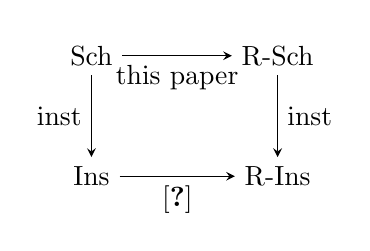
\begin{tikzpicture}
    \centering \matrix (m) [matrix of math nodes,row sep=3em,column
    sep=4em,minimum width=2em] {
      \text{Sch} & \text{R-Sch} \\
      \text{Ins} & \text{R-Ins} \\}; \path[-stealth] (m-1-1) edge node [left]
    {inst} (m-2-1) edge node [below] {this paper} (m-1-2)
    (m-2-1.east|-m-2-2) edge node [below] {\cite{LaneseM20}} node [] {} (m-2-2)
    (m-1-2) edge node [right] {inst} (m-2-2);
  \end{tikzpicture}
  \caption{ Schema of the proof of correctness. }
  \label{fig:square}
\end{figure}

This is part of our ongoing work.

%% \section{Related}\label{sec:related}
%% First, in~\cite{Gonzalez-AbrilV21} the expression semantics is not directly
%% defined on expressions, but on an
%% operator $C[\bullet]$, which is used to select the part of the expression that has to be
%% evaluated, however no definition of such operator is given.

%% In Maude, since the semantics is
%% runnable, we need to define every operator. So, we opted for an approach closer
%% to the one in~\cite{LaneseNPV18}, where we have rules that recursively evaluate
%% the expression until a computation is executed - as already discussed, we can use
%% conditional equations to first perform operations and then use others equations
%% to further reduce.


%% For example, if the expression under evaluation is
%% $\ms{case}~foo(42)~\ms{of}\ldots$ the context operator would put automatically
%% the focus on $foo(42)$, i.e., $C[foo(42)]$. The convenience of using such
%% operator is that in this way one can avoid the definition of all the rules to
%% evaluate inner parts of an expression, like in the example just presented.

%% To avoid these problems the solution adopted
%% in~\cite{Gonzalez-AbrilV21} is to push the current environment together with the
%% context operator, where the term under evaluation is replaced with a
%% placeholder, in a stack and to start a new subcomputation - with the appropriate
%% environment. Then, once the
%% subcomputation is over the old contest and environment are retrieved from the
%% stack and the final value of the subcomputation is replaced inside the expression
%% which gave rise to it.

%% Again the context operators makes the formalization of this mechanism
%% much easier. Indeed in reality, to implement such approach it would be necessary to define, for each supported construct, a rule to start the subcomputation and another rule to replace the
%% value once the subcomputation is over.

%% To address the problem the solution proposed in~\cite{Gonzalez-AbrilV21},
%% already used in~\cite{LaneseNPV18}, is to evaluate those rules that need some information
%% available at the system level to a symbol $\kappa$, in other words a
%% \emph{future}. Then, the duty of replacing $\kappa$ with the
%% appropriate information is delegated to the system level.

%% The final difference between our semantics and the one proposed
%% in~\cite{Gonzalez-AbrilV21} concerns those rules of the expression semantics
%% that need to rely on some information held by the system level. This is the case
%% for instance for the $\ms{self}$ primitive or the $\ms{receive}$ statement, in
%% the first case the information required is the process pid, held in the process
%% tuple, and in the second case the information required is the message which has
%% to be received.



\section{Conclusion}\label{sec:conclusion}
We presented a new formalization of the Erlang language using Maude.
Having a mechanized version of the Erlang semantics makes it much easier to
debug it and to become confident that the semantics correctly captures the
behavior of the language. Indeed, to test the semantics, in our work, one can
load an Erlang module and actually run an arbitrary program (as long as
the program uses supported primitives) and the states traversed can be
compared against an actual execution to make sure that the two agree.

Concretely, defining an executable semantics of a language poses also
some challenges that do not rise for arbitrary semantics. For
instance, the semantics in~\cite{Gonzalez-AbrilV21} resorts to the
existence of suitable contexts to identify the redex inside an
expression, while we need to explicitly give an inductive definition
to find the redex.

We also implemented a program able to transform a non-reversible
semantics into a reversible one, providing an implementation of the
general method described in~\cite{LaneseM20}. Again, ensuring that the
method can be actually executed poses some challenges.
E.g.,~\cite{LaneseM20} just declares that
keys are generated fresh, while we had to provide a concrete and
distributed algorithm to generate keys ensuring their freshness.

Let us now discuss possible future improvements for the presented
work. First, one could investigate ways to optimize the implementation
of the semantics, so to be able to simulate more computationally
expensive Erlang computations. For instance, right now the top-level
environment also includes the bindings from the lower levels, and this
increases the needed memory.  Second, one could support further
primitives to widen the set of executable programs. In doing so it is
important to make sure that the causal-dependencies captured by the
producer-consumer model used in~\cite{LaneseM20} are appropriate - for
example the model is not well-suited to capture dependencies due to
shared memory.

\bibliographystyle{unsrt}
\bibliography{references.bib}

\end{document}
